\documentclass[a4paper,11pt]{article}
\usepackage{amsmath,amsthm,amsfonts,amssymb,amscd,amstext,vmargin,graphics,graphicx,tabularx,multicol} \usepackage[french]{babel}
\usepackage[utf8]{inputenc}  
\usepackage[T1]{fontenc} 
\usepackage[T1]{fontenc}
\usepackage{amsmath,amssymb}
\usepackage{pstricks-add,tikz,tkz-tab,variations}
\usepackage[autolanguage,np]{numprint} 

\setmarginsrb{1.5cm}{0.5cm}{1cm}{0.5cm}{0cm}{0cm}{0cm}{0cm} %Gauche, haut, droite, haut
\newcounter{numexo}
\newcommand{\exo}[1]{\stepcounter{numexo}\noindent{\bf Exercice~\thenumexo} : \marginpar{\hfill /#1}}
\reversemarginpar


\newcounter{enumtabi}
\newcounter{enumtaba}
\newcommand{\q}{\stepcounter{enumtabi} \theenumtabi.  }
\newcommand{\qa}{\stepcounter{enumtaba} (\alph{enumtaba}) }
\newcommand{\initq}{\setcounter{enumtabi}{0}}
\newcommand{\initqa}{\setcounter{enumtaba}{0}}

\newcommand{\be}{\begin{enumerate}}
\newcommand{\ee}{\end{enumerate}}
\newcommand{\bi}{\begin{itemize}}
\newcommand{\ei}{\end{itemize}}
\newcommand{\bp}{\begin{pspicture*}}
\newcommand{\ep}{\end{pspicture*}}
\newcommand{\bt}{\begin{tabular}}
\newcommand{\et}{\end{tabular}}
\renewcommand{\tabularxcolumn}[1]{>{\centering}m{#1}} %(colonne m{} centrée, au lieu de p par défault) 
\newcommand{\tnl}{\tabularnewline}

\newcommand{\trait}{\noindent \rule{\linewidth}{0.2mm}}
\newcommand{\hs}[1]{\hspace{#1}}
\newcommand{\vs}[1]{\vspace{#1}}

\newcommand{\N}{\mathbb{N}}
\newcommand{\Z}{\mathbb{Z}}
\newcommand{\R}{\mathbb{R}}
\newcommand{\C}{\mathbb{C}}
\newcommand{\Dcal}{\mathcal{D}}
\newcommand{\Ccal}{\mathcal{C}}
\newcommand{\mc}{\mathcal}

\newcommand{\vect}[1]{\overrightarrow{#1}}
\newcommand{\ds}{\displaystyle}
\newcommand{\eq}{\quad \Leftrightarrow \quad}
\newcommand{\vecti}{\vec{\imath}}
\newcommand{\vectj}{\vec{\jmath}}
\newcommand{\Oij}{(O;\vec{\imath}, \vec{\jmath})}
\newcommand{\OIJ}{(O;I,J)}

\newcommand{\bmul}[1]{\begin{multicols}{#1}}
\newcommand{\emul}{\end{multicols}}


\newcommand{\reponse}[1][1]{%
\multido{}{#1}{\makebox[\linewidth]{\rule[0pt]{0pt}{20pt}\dotfill}
}}

\newcommand{\titre}[5] 
% #1: titre #2: haut gauche #3: bas gauche #4: haut droite #5: bas droite
{
\noindent #2 \hfill #4 \\
#3 \hfill #5

\vspace{-1.6cm}

\begin{center}\rule{6cm}{0.5mm}\end{center}
\vspace{0.2cm}
\begin{center}{\large{\textbf{#1}}}\end{center}
\begin{center}\rule{6cm}{0.5mm}\end{center}
}



\begin{document}
\pagestyle{empty}
\titre{Correction du Contrôle 2 : Fractions (Chp 1 et 2), probabilités et symétrie centrale }{5ème}{}{}{}



\exo{5}

Calculer les expressions suivantes en détaillant toutes vos étapes de calculs et \textbf{simplifier} les résultats si besoin :

\red

\bmul{4}

$R = \dfrac{4}{5} + \dfrac{18}{5}$\\
$R = \dfrac{4+18}{5} $\\
\fbox{$R = \dfrac{22}{5} $}\\

\columnbreak

$E = \dfrac{5}{3} - \dfrac{10}{12}$\\

$E = \dfrac{5 \times 4}{3 \times 4} - \dfrac{10}{12}$\\ 

$E = \dfrac{20}{12} - \dfrac{10}{12}$\\ 

$E = \dfrac{20 - 10}{12}$\\

$E = \dfrac{10 \div 2}{12 \div 2}$\\

\fbox{$E = \dfrac{5}{6}$}\\

\columnbreak

$P = \dfrac{3}{1} - \dfrac{2}{7}$\\ 

$P = \dfrac{3 \times 7}{1 \times 7} - \dfrac{2}{7}$\\ 

$P = \dfrac{21}{7} - \dfrac{2}{7}$\\ 

\fbox{$P = \dfrac{19}{7}$}\\ 


\columnbreak

$S =\dfrac{1 }{3}+\dfrac{4}{5} - \dfrac{11}{45}$\\
 
$S =\dfrac{1\times 15}{3\times 15}+\dfrac{4\times 9}{5\times 9} - \dfrac{11}{45}$\\

$S =\dfrac{15}{45}+\dfrac{36}{45} - \dfrac{11}{45}$\\ 

$S =\dfrac{15 + 36 - 11}{45}$\\ 

$S =\dfrac{40 \div 5}{45 \div 5}$\\ 

\fbox{$S =\dfrac{8}{9}$}\\ 


\emul

\vspace*{0.5cm}

\black \exo{2}

\red \underline{Quantité de boisson :}\\

$\dfrac{1}{2} + \dfrac{1}{10} +\dfrac{1}{20} + \dfrac{2}{5}  =\dfrac{1 \times 10}{2 \times 10} + \dfrac{1 \times 2}{10 \times 2} +\dfrac{1}{20} + \dfrac{2 \times 4}{5 \times 4}$\\

$= \dfrac{10}{20} + \dfrac{2}{20} +\dfrac{1}{20} + \dfrac{8}{20}$
$= \dfrac{21}{20}$ L\\

Or, $\dfrac{21}{20} \textrm{L} > 1 \textrm{L} $. Donc la carafe va bien déborder.\\



\black \exo{2,5}

On prend deux dés cubiques non truqués. On les lance et on ajoute les deux nombres obtenus.

\initq \q Est-ce une expérience aléatoire ? (\textbf{Justifier votre réponse)}

\red Oui c'est une expérience aléatoire car on peut la reproduire plusieurs fois dans les même conditions et on ne peut pas prévoir le résultat.\\

\black \q Combien y a-t-il d'issues possibles ? Citer-les.

\red Il y a 11 issues possibles : "Obtenir 2", "Obtenir 3", "Obtenir 4", "Obtenir 5",  "Obtenir 6", "Obtenir 7", "Obtenir 8", "Obtenir 9", "Obtenir 10" et "Obtenir 11".



\vspace*{0.5cm}

\black \exo{1}

Lucie dit qu'elle a lancé six fois de suite un dé à six faces non truqué et elle affirme qu'elle a obtenu à chaque fois le chiffre 5.

\initq \q Est-ce possible ?(\textbf{Justifier votre réponse)}

\red Oui, c'est possible. L'expérience est une expérience aléatoire donc on ne peut prévoir le résultat. \\

\black \q Si Lucie relance le dé, a-t-elle une chance de refaire un 5 ?(\textbf{Justifier votre réponse)}

\red Oui, car dans cette expérience, on a autant de chance de tomber sur le 5 qu'un autre chiffre.\\

\vspace*{0.5cm}

\black \exo{1,5} 

\red 

\bi

\item $1^{er}$ cas : Si on choisi la roulette, on a 3 chances sur 8 d'obtenir du rouge, soit $\dfrac{3}{8}$.

\item $2^{eme}$ cas : Si on choisi le dé, on a 2 chances sur 6, d'obtenir du rouge, soit $\dfrac{2}{6} = \dfrac{1}{3}$.

\item $3^{eme}$ cas : Si on choisi l'urne, on a 4 chances sur 10 d'obtenir du rouge, soit $\dfrac{4}{10} = \dfrac{2}{5}$\\

\ei


Comparons les fractions suivantes :\\

$ \dfrac{3}{8} = \dfrac{3\times 15}{8 \times 15} $
$= \dfrac{45}{120}$\\

$ \dfrac{1}{3} = \dfrac{1\times 40}{3 \times 40} $
$= \dfrac{40}{120}$\\

$ \dfrac{4}{10} = \dfrac{4\times 12}{10 \times 12} $
$= \dfrac{48}{120}$\\

La fraction la plus grande est $ \dfrac{48}{120}$, donc on a plus de chance de gagner en choisissant l'urne.

\vspace*{0.5cm}



\black \exo{3} Dans la figure ci-dessous, les quadrilatères ACBD et EFHG sont symétriques par rapport au point O.


\initq

\black \q Quel est le symétrique de point B par rapport au point O.

\red Le symétrique du point B par rapport au point O est E.\\

\black \q Quel est le symétrique du segment [AD] par rapport au point O.

\red Le symétrique du segment [AD] par rapport au point O est [HG].\\

\black \q Quel est le symétrique de la droite (FH) par rapport au point O.

\red Le symétrique de la droite (FH) par rapport au point O est (CA).\\

\black \q Quel est le symétrique de la droite (FG) par rapport au point O.

\red Le symétrique de la droite (FG) par rapport au point O est (CD).\\

\vspace*{0.5cm}

\black \exo{2}

Après avoir reproduit ce dessin sur \textbf{ta copie}, complète-le en faisant le symétrique de chaque figure par rapport au point O.\\

\begin{center}
\includegraphics[scale=1]{figure.eps} 
\end{center}

\vspace*{0.5cm}

\exo{3} \initq 
\q Construire un triangle ABC rectangle en A tel que  : AB = 5cm et AC = 3cm.\\
\q Construire le symétrique du segment [BC] par rapport au point A.\\
\q Construire le symétrique de la droite (AB) par rapport au point C.


\end{document}
